\documentclass[conference]{IEEEtran}
\IEEEoverridecommandlockouts

\usepackage{cite}
\usepackage{amsmath,amssymb,amsfonts}
\usepackage{graphicx}
\usepackage{textcomp}
\usepackage{xcolor}
\usepackage{booktabs}
\usepackage{array}
\usepackage[utf8]{inputenc}
\usepackage[T1]{fontenc}
\graphicspath{{figs/mlp/}}

\def\BibTeX{{\rm B\kern-.05em{\sc i\kern-.025em b}\kern-.08em
    T\kern-.1667em\lower.7ex\hbox{E}\kern-.125emX}}

\begin{document}

\title{Classificação de Áreas Queimadas com\\
Multilayer Perceptron (MLP)}

\author{
  \IEEEauthorblockN{Autor}
  \IEEEauthorblockA{
    \textit{Reconhecimento de Padrões}\\
    Sensoriamento Remoto Orbital $\cdot$ Landsat~8/9\\
    Treino: 220\_075 + 221\_074 $\cdot$ Teste: 222\_074 $\cdot$ Agosto de 2024
  }
}

\maketitle

\begin{abstract}
Rede neural MLP em PyTorch com \textbf{10 features espectrais} (B4, B5, B7,
NDVI e NBR — pré e pós-queimada) foi treinada nas cenas Landsat~8/9
220\_075 e 221\_074 e avaliada de forma cega na cena 222\_074 (40,3~milhões
de pixels, 2,96\% queimada). Hiperparâmetros otimizados por Optuna
(5~\textit{trials}) resultaram em arquitetura de 2~camadas $\times$ 64~neurônios
com Adam e Dropout~$= 0{,}256$. A validação cruzada estratificada 5-fold
(cenas treino) atingiu $F_1 = 0{,}722 \pm 0{,}002$ e
$\mathrm{AUC} = 0{,}812 \pm 0{,}002$; no teste cego,
$\mathrm{AUC} = 0{,}830$ e Recall~$= 0{,}713$, indicando boa capacidade
discriminativa com precisão limitada pelo forte desequilíbrio de classes (97:3)
na cena de teste.
\end{abstract}

\begin{IEEEkeywords}
área queimada, MLP, rede neural, PyTorch, Optuna, Landsat, sensoriamento
remoto, validação cruzada, desbalanceamento de classes.
\end{IEEEkeywords}

%=====================================================================
\section{Problema, Entradas e Saída do Modelo}

\textbf{Objetivo:} classificar cada pixel de uma imagem de satélite Landsat~8/9
(resolução 30~m) em uma de duas classes: \textbf{Classe~0 — Não queimada}
$|$ \textbf{Classe~1 — Queimada}.

A Tabela~\ref{tab:io} resume o fluxo de entrada e saída do modelo.

\begin{table}[!t]
  \caption{Entradas e saídas da MLP}
  \label{tab:io}
  \centering
  \begin{tabular}{ll}
    \toprule
    \textbf{ENTRADA} & \textbf{SAÍDA} \\
    \midrule
    10 valores por pixel & Probabilidade de cada classe \\
    Pré-queimada: B4, B5, B7, NDVI, NBR & $\hat{p}(\text{queimada})$ \\
    Pós-queimada: B4, B5, B7, NDVI, NBR & $\hat{p}(\text{não queimada})$ \\
    (normalizados por \texttt{StandardScaler}) & (via Softmax + limiar 0,5) \\
    \bottomrule
  \end{tabular}
\end{table}

%=====================================================================
\section{Metodologia}

\subsection{Dados, Protocolo e Desbalanceamento}

Foram utilizadas três cenas Landsat~8/9 (Coleção~2, reflectância de
superfície, agosto de 2024):
\begin{itemize}
  \item \textbf{220\_075} (LC09, 29/08): treino e validação;
  \item \textbf{221\_074} (LC08, 28/08): treino e validação;
  \item \textbf{222\_074} (LC09, 27/08): teste cego.
\end{itemize}

\textbf{Protocolo treino/val/teste:}
\begin{itemize}
  \item \textbf{Treino + Validação}: cenas 220\_075 e 221\_074 — 100k pixels
        por classe de cada cena $= 400$k pixels totais (balanceados 50/50).
  \item \textbf{Validação}: Stratified 5-Fold CV no conjunto de treino,
        preservando proporção de classes em cada fold.
  \item \textbf{Teste cego}: todos os 40,3~M pixels válidos da cena 222\_074
        (2,96\% queimada), nunca vistos durante treino.
\end{itemize}

O dataset completo apresenta razão de até 18:1 entre classes, justificando
a amostragem balanceada e o uso de \texttt{class\_weight} na função de perda.
A Fig.~\ref{fig:distribuicao} ilustra essa distribuição.

\begin{figure}[!t]
  \centering
  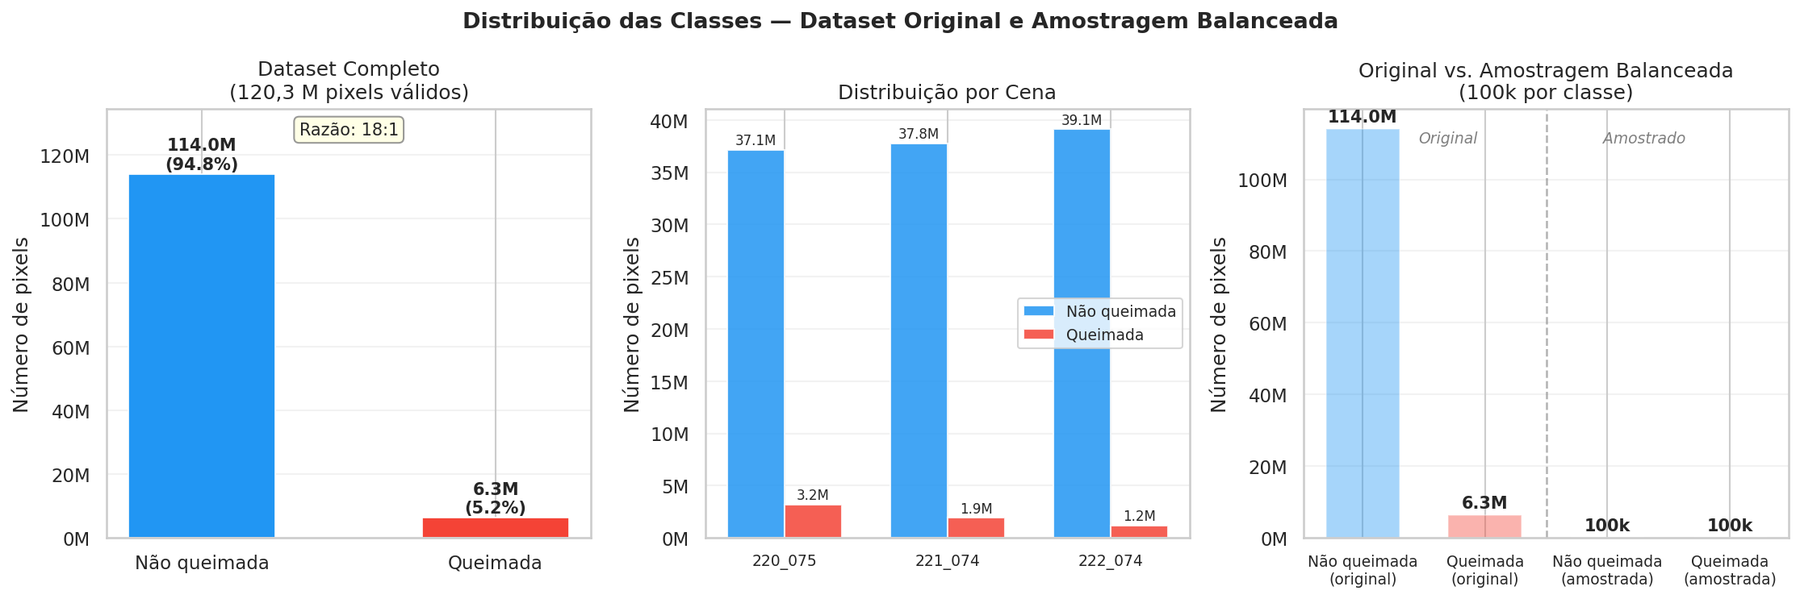
\includegraphics[width=\columnwidth]{fig_distribuicao.png}
  \caption{Distribuição das classes: dataset completo (esq.), por cena (centro)
           e amostragem balanceada 100k/classe (dir.). Razão original 18:1.}
  \label{fig:distribuicao}
\end{figure}

\subsection{Arquitetura e Treinamento}

A Tabela~\ref{tab:arch} descreve a arquitetura da rede neural utilizada.

\begin{table}[!t]
  \caption{Arquitetura da MLP}
  \label{tab:arch}
  \centering
  \begin{tabular}{ll}
    \toprule
    \textbf{Componente} & \textbf{Especificação} \\
    \midrule
    Entrada       & 10 neurônios (B4, B5, B7, NDVI, NBR $\times$ pré+pós) \\
    Camadas ocultas & $2 \times 64$ — BatchNorm1d + ReLU + Dropout(0,256) \\
    Saída         & 2 logits $\rightarrow$ CrossEntropyLoss com pesos \\
    Anti-leakage  & StandardScaler fitado somente nos dados de treino \\
    Regularização & Early Stopping (paciência~10); Dropout estocástico \\
    \bottomrule
  \end{tabular}
\end{table}

A otimização de hiperparâmetros foi realizada com \textbf{Optuna TPE Sampler}
(5~\textit{trials}, \texttt{MedianPruner}), minimizando a \textit{val\_loss}.
Parâmetros fixos: Adam ($\alpha = 10^{-3}$), batch~1024, $n_{\text{epochs}} \leq 50$.

%=====================================================================
\section{Resultados}

\subsection{Validação Cruzada — Métricas por Fold}

A Tabela~\ref{tab:cv} apresenta os resultados da validação cruzada
estratificada 5-fold. Métricas referem-se à classe queimada (positiva).

\begin{table}[!t]
  \caption{Stratified 5-Fold CV — Cenas 220\_075 + 221\_074 (400k pixels)}
  \label{tab:cv}
  \centering
  \begin{tabular}{cccccc}
    \toprule
    \textbf{Fold} & \textbf{Acc.} & \textbf{Prec.} & \textbf{Recall}
                  & \textbf{F1} & \textbf{AUC-ROC} \\
    \midrule
    1 & 0,7309 & 0,7454 & 0,7013 & 0,7227 & 0,8099 \\
    2 & 0,7317 & 0,7564 & 0,6835 & 0,7181 & 0,8114 \\
    3 & 0,7321 & 0,7472 & 0,7017 & 0,7237 & 0,8108 \\
    4 & 0,7345 & 0,7586 & 0,6880 & 0,7216 & 0,8143 \\
    5 & 0,7342 & 0,7563 & 0,6912 & 0,7223 & 0,8135 \\
    \midrule
    \textbf{Média} & \textbf{0,7327} & \textbf{0,7528} & \textbf{0,6931}
                   & \textbf{0,7217} & \textbf{0,8120} \\
    \textbf{DP}    & 0,0015 & 0,0055 & 0,0079 & 0,0022 & 0,0019 \\
    \bottomrule
  \end{tabular}
\end{table}

Os resultados apresentam baixo desvio padrão entre os folds, indicando
estabilidade do modelo e ausência de overfitting durante o treinamento.
A Fig.~\ref{fig:curvas} mostra as métricas por fold e a curva de loss média.

\begin{figure}[!t]
  \centering
  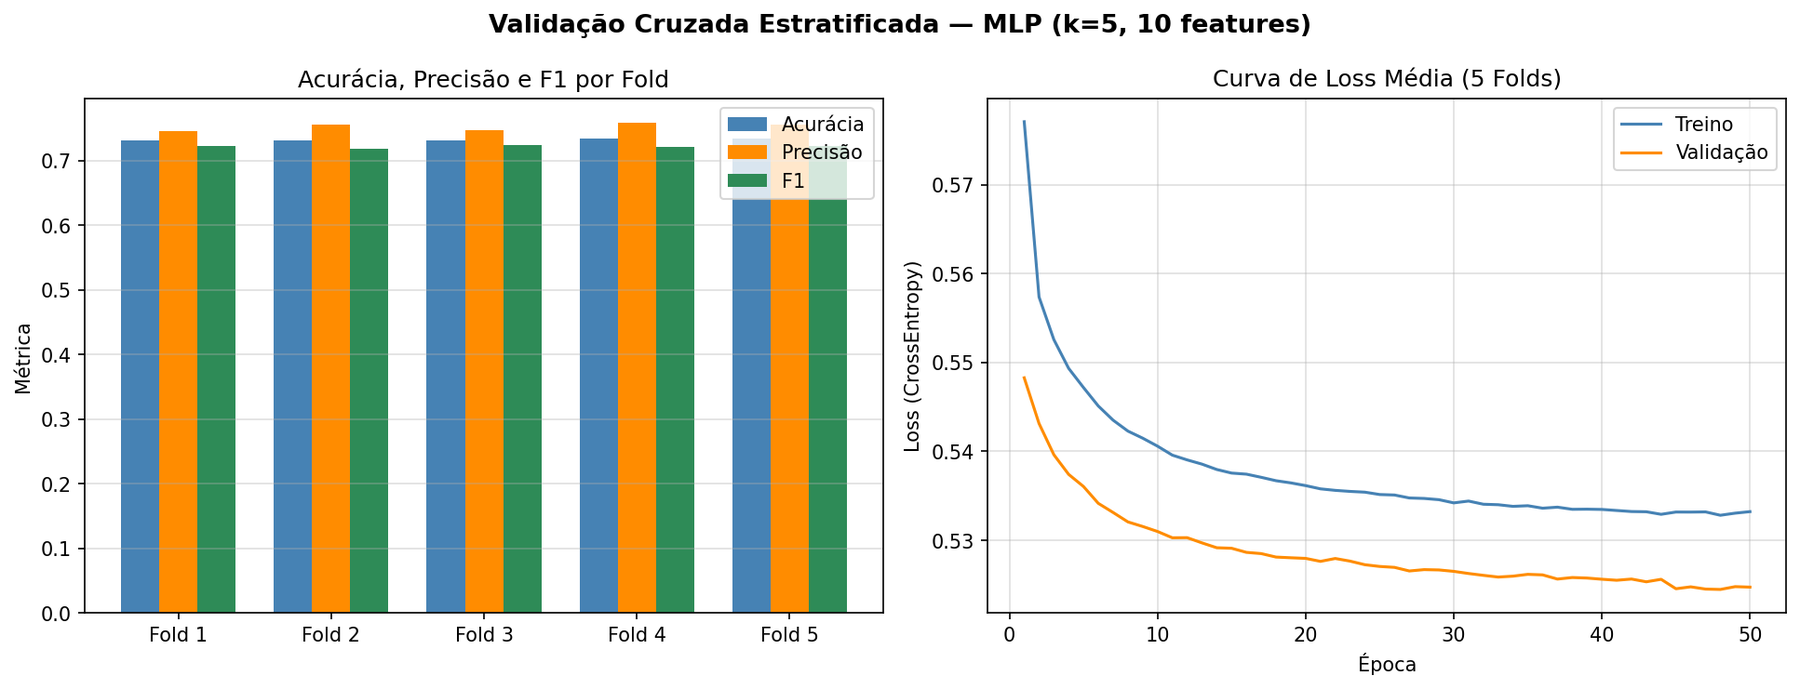
\includegraphics[width=\columnwidth]{fig_curvas_val.png}
  \caption{Validação cruzada estratificada ($k=5$, 10~features): accuracy,
           precision e F1 por fold (esq.) e curva de loss média (dir.).}
  \label{fig:curvas}
\end{figure}

\subsection{Teste Cego — Cena 222\_074}

A Tabela~\ref{tab:test} compara os resultados da validação cruzada com o
teste cego completo na cena 222\_074 (40,3~M pixels).

\begin{table}[!t]
  \caption{Comparação validação cruzada vs.\ teste cego}
  \label{tab:test}
  \centering
  \setlength{\tabcolsep}{4pt}
  \begin{tabular}{lccccc}
    \toprule
    \textbf{Conjunto / Modelo} & \textbf{Acc.} & \textbf{Prec.}
                               & \textbf{Recall} & \textbf{F1} & \textbf{AUC} \\
    \midrule
    MLP — Val.\ cruzada (média) & 0,733 & 0,753 & 0,693 & 0,722 & 0,812 \\
    MLP — Teste 222\_074 (40M)  & 0,830 & 0,116 & 0,713 & 0,199$^{*}$ & 0,830 \\
    \bottomrule
    \multicolumn{6}{l}{$^{*}$Precision baixa. AUC indica separabilidade real.}
  \end{tabular}
\end{table}

\subsection{Matriz de Confusão}

A Tabela~\ref{tab:cm} apresenta os valores absolutos da matriz de confusão
no teste cego.

\begin{table}[!t]
  \caption{Matriz de Confusão — Cena 222\_074 (Teste Cego)}
  \label{tab:cm}
  \centering
  \begin{tabular}{lcc}
    \toprule
    & \textbf{Pred.\ Não Queimada} & \textbf{Pred.\ Queimada} \\
    \midrule
    \textbf{Real Não Queimada} & 32.615.748 (TN) & 6.492.125 (FP) \\
    \textbf{Real Queimada}     &    342.867 (FN) &   851.109 (TP) \\
    \bottomrule
  \end{tabular}
\end{table}

\begin{figure}[!t]
  \centering
  \begin{minipage}[b]{0.48\columnwidth}
    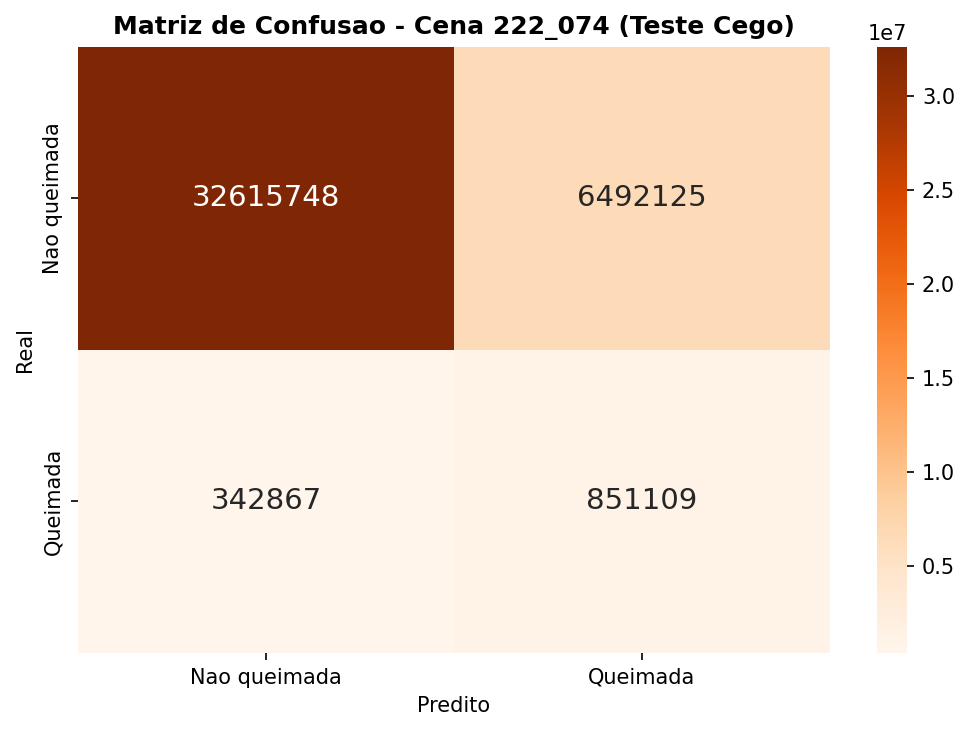
\includegraphics[width=\textwidth]{fig_cm.png}
    \caption*{(a) Matriz de Confusão}
  \end{minipage}
  \hfill
  \begin{minipage}[b]{0.48\columnwidth}
    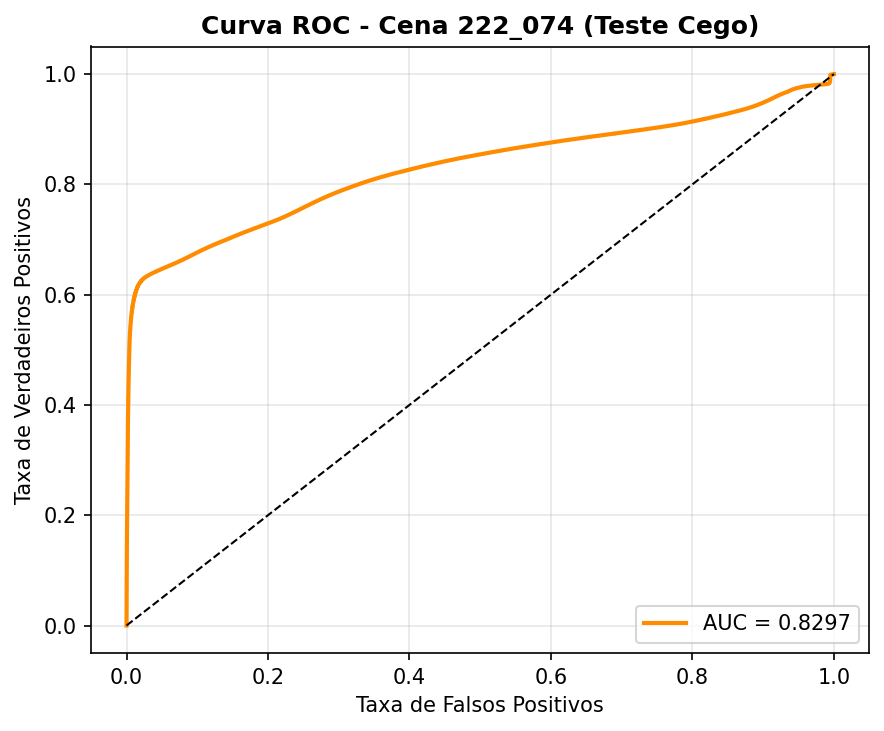
\includegraphics[width=\textwidth]{fig_roc.png}
    \caption*{(b) Curva ROC}
  \end{minipage}
  \caption{Teste cego 222\_074: (a) CM — TN=32,6M, FP=6,5M, FN=343k,
           TP=851k; (b) Curva ROC — AUC=0,830.}
  \label{fig:cm_roc}
\end{figure}

%=====================================================================
\section{Discussão}

\subsection{Desempenho na Validação vs.\ Teste Cego}

A diferença entre as métricas de validação cruzada ($F_1 = 0{,}722$,
Precision~$= 0{,}753$) e o teste cego ($F_1 = 0{,}199$, Precision~$= 0{,}116$)
é esperada: o treinamento utilizou amostragem balanceada 50/50, enquanto a
cena de teste apresenta apenas 2,96\% de pixels queimados (razão 97:3). O
AUC~$= 0{,}830$ no teste cego confirma que o modelo discrimina bem as classes
no espaço de probabilidade — a queda no F1 é consequência do desbalanceamento
e do limiar fixo em 0,5.

\subsection{Curva de Aprendizado}

A curva de \textit{loss} média dos 5~folds demonstra convergência saudável:
a \textit{val\_loss} decresce e se estabiliza antes do critério de Early
Stopping, sem divergência, indicando arquitetura adequada à complexidade
do problema.

\subsection{Limitações}

A principal limitação reside na confusão entre solos expostos e cicatrizes de
queimada recente, problema compartilhado com todos os métodos que utilizam
apenas assinatura espectral multitemporal sem índice de diferença. O uso de
$\Delta$NBR e $\Delta$NDVI como \textit{features} pode melhorar
significativamente a separabilidade, desde que a máscara de referência seja
derivada de fonte independente.

%=====================================================================
\section{Conclusão}

A MLP (2~camadas $\times$ 64~neurônios, Adam, Dropout~$= 0{,}256$,
10~features) atingiu $F_1 = 0{,}722$ e $\mathrm{AUC} = 0{,}812$ na
validação cruzada, sem \textit{overfitting}. No teste cego 222\_074,
$\mathrm{AUC} = 0{,}830$ confirma separabilidade espectral, mas a Precision
cai para 0,116 com limiar 0,5 — consequência do treino balanceado (50/50)
aplicado a uma cena com 2,96\% de queimada. Ajuste de threshold via curva
Precision-Recall poderia equilibrar melhor as métricas para esta aplicação.

\begin{thebibliography}{00}

\bibitem{b1}
E.~Chuvieco \textit{et al.},
``Generation and analysis of a new global burned area product based on
MODIS 250~m reflectance bands,''
\textit{Earth System Science Data}, vol.~11, pp.~529--551, 2019.

\bibitem{b2}
C.~H.~Key e N.~C.~Benson,
``Landscape Assessment: Composite Burn Index,''
in \textit{FIREMON}, USDA Forest Service, RMRS-GTR-164-CD, 2006.

\bibitem{b3}
Y.~LeCun, Y.~Bengio e G.~Hinton,
``Deep learning,''
\textit{Nature}, vol.~521, pp.~436--444, 2015.

\bibitem{b4}
J.~Bergstra \textit{et al.},
``Algorithms for hyper-parameter optimization,''
\textit{NeurIPS}, vol.~24, pp.~2546--2554, 2011.

\end{thebibliography}

\end{document}
